\documentclass[aspectratio=169]{beamer}

\usetheme{default}
\usecolortheme{dolphin}
\setbeamertemplate{navigation symbols}{}
\setbeamertemplate{footline}[frame number]
\setbeamerfont{frametitle}{size=\large}
\setbeamercolor{frametitle}{fg=black}

\usepackage{graphicx}
\usepackage{booktabs}
\usepackage{amsmath}
\usepackage{bm}

\title{Bounding VIO Drift with Self-Supervised Aerial Geo-Localization}
\subtitle{GNSS-denied UAV navigation, CPU-only}
\author{Nijat Abbasov}
\date{\today}

\begin{document}

\begin{frame}
\titlepage
\end{frame}

%---------------------------------------------------------------- 1. abstract
\begin{frame}{The problem, and the result}
\textbf{Two estimators with opposite failure modes.}
\begin{itemize}
\item \textbf{VIO} (OpenVINS) --- smooth, locally accurate, \emph{drifts without
      bound}. On this flight: 700\,m over 3.6\,km, 19\% of distance flown.
\item \textbf{Geo-localization} (CAEVL) --- absolute, \emph{never drifts}, but
      only 36\% of predictions are correct and its confidence score cannot tell
      you which.
\end{itemize}

\vspace{0.4em}
\textbf{Result} --- MUN-FRL \texttt{bell412\_dataset4}, 3.6\,km over Ottawa
International Airport:

\vspace{0.3em}
\centering
\begin{tabular}{@{}lccc@{}}
\toprule
 & OpenVINS & Fused & \\
\midrule
Real-time (causal) RMSE & 540\,m & \textbf{347\,m} & $-36\%$ \\
Offline, cruise only    & 166\,m & \textbf{48\,m}  & $-71\%$ \\
\bottomrule
\end{tabular}

\vspace{0.6em}
\raggedright
Everything runs on \textbf{CPU}: retrieval 233\,ms/query, VIO at 20\,Hz.
\end{frame}

%------------------------------------------------------- 2. CAEVL + OpenVINS
\begin{frame}{CAEVL --- self-supervised geo-localization}
\begin{columns}[T]
\begin{column}{0.52\textwidth}
\textbf{The domain gap:} a photo taken now versus satellite imagery from months
ago --- different sensor, season, sun angle.

\vspace{0.5em}
\textbf{The trick:} throw appearance away. Both sides become \textbf{Canny edge
maps} --- roads and field boundaries survive, colour and illumination do not.

\vspace{0.5em}
\textbf{Training, on reference imagery \emph{only}:}
\begin{enumerate}
\item Autoencoder, edge map $\rightarrow$ 1024-d descriptor, with a DINOv2
      perceptual loss
\item VICReg fine-tuning on (clean tile, degraded copy) pairs --- no negatives,
      no paired UAV data
\end{enumerate}

\vspace{0.5em}
Deploying over new terrain needs \textbf{satellite tiles and nothing else}.
\end{column}
\begin{column}{0.46\textwidth}
\centering
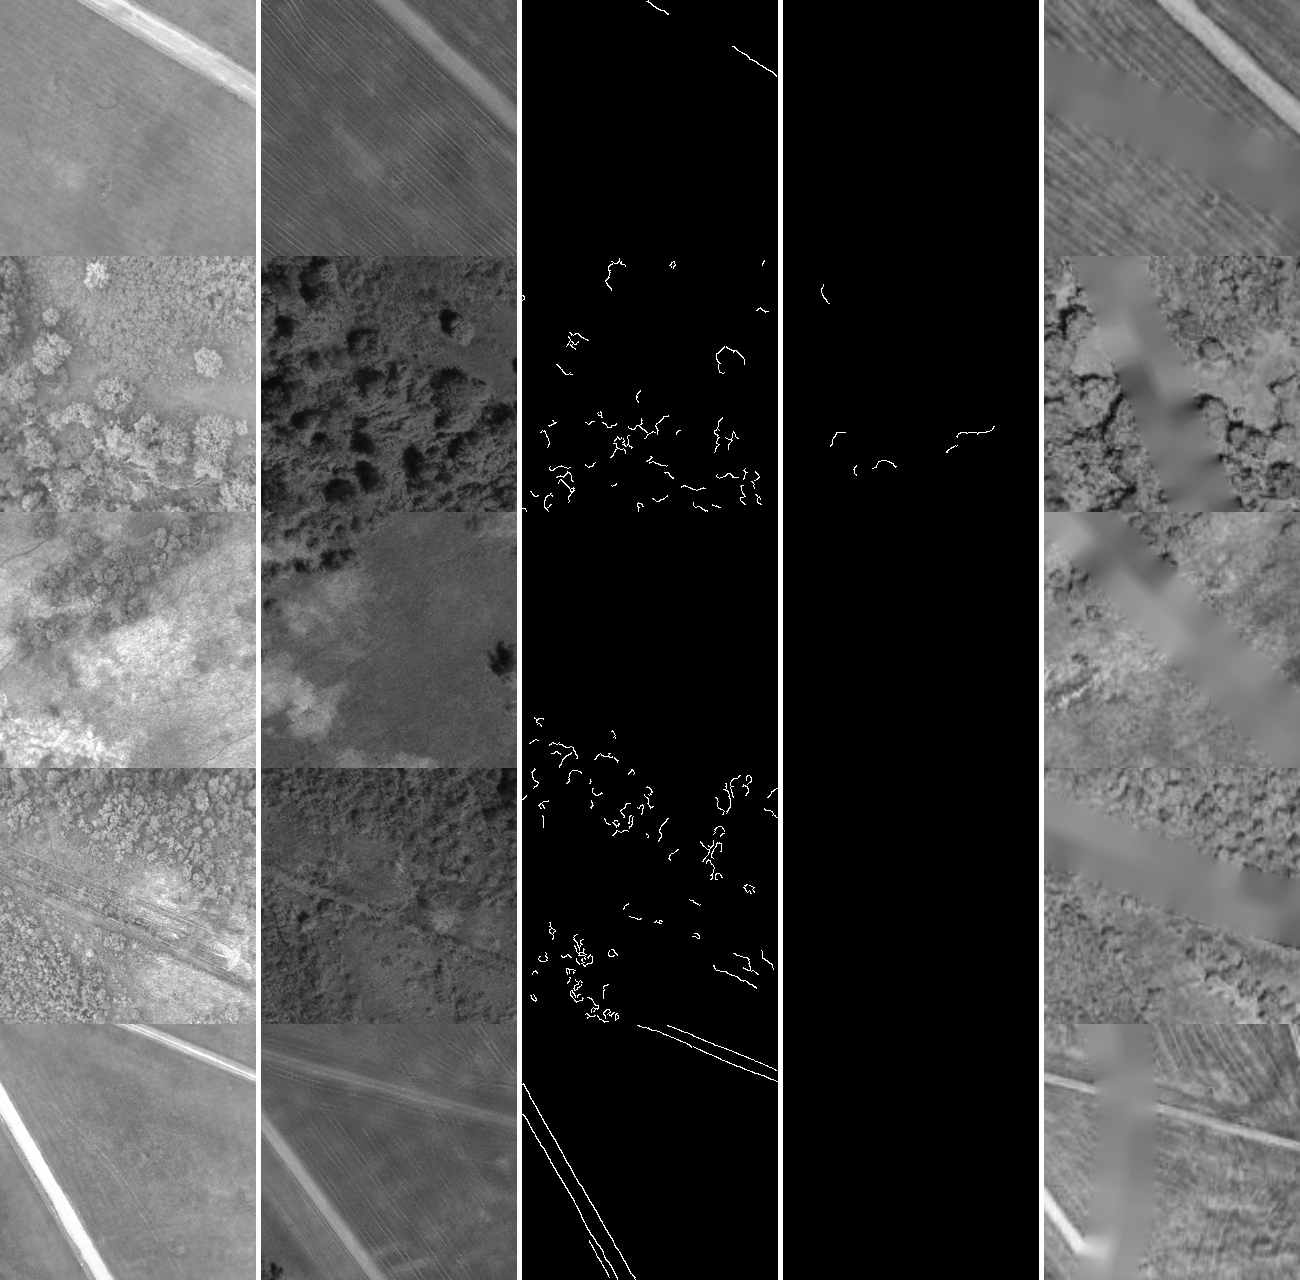
\includegraphics[width=\linewidth]{figures/esri_vs_munfrl.png}\\
{\scriptsize query \quad tile \quad their Canny edges}

\vspace{0.5em}
\begin{tabular}{@{}lc@{}}
\toprule
ViLD reproduction & R@1 \\
\midrule
Paper & 49.68\% \\
Ours & 48.14\% \\
\quad + perceptual loss & \textbf{52.88\%} \\
\bottomrule
\end{tabular}
\end{column}
\end{columns}
\end{frame}

\begin{frame}{OpenVINS --- and why the dataset was hard to find}
\begin{columns}[T]
\begin{column}{0.46\textwidth}
MSCKF visual-inertial odometry, monocular, nadir camera. \textbf{No loop
closure} --- landmarks are marginalised.

\vspace{0.5em}
Anchored at takeoff it starts 14.7\,m from truth and drifts to \textbf{700\,m}.
A best-fit scale correction recovers it to 215\,m, so most of the error is a
systematic \textbf{40\% scale deficit}, not random walk.

\vspace{0.8em}
\textbf{Why MUN-FRL:} the two halves want opposite flight profiles ---
\begin{itemize}
\item VIO needs \textbf{parallax} $\rightarrow$ fly low
\item Geo-localization needs \textbf{ground footprint} $\rightarrow$ fly high
\end{itemize}
so datasets optimise for one or the other.
\end{column}
\begin{column}{0.52\textwidth}
\centering
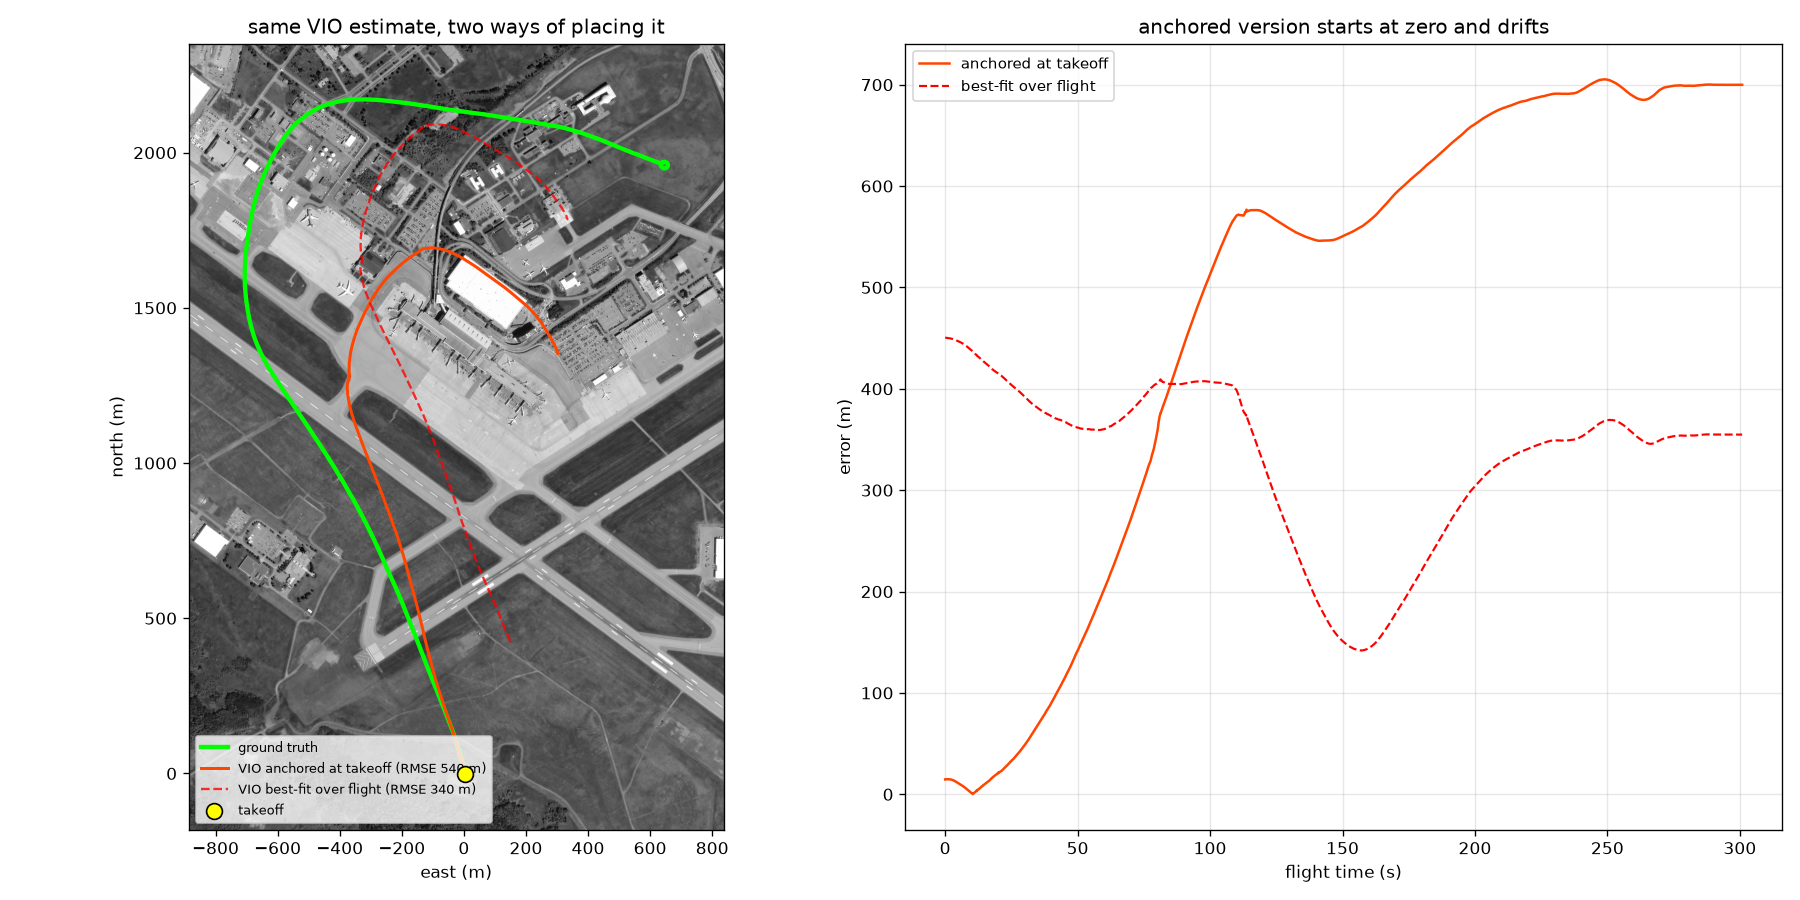
\includegraphics[width=\linewidth]{figures/vio_anchoring_dataset4.png}

\vspace{0.3em}
{\scriptsize
\begin{tabular}{@{}llc@{}}
\toprule
Dataset & Altitude & IMU \\
\midrule
VPAIR & 300\,m & no \\
AerialVL & --- & no \\
SatLoc & 100--300\,m & not released \\
Zurich MAV & 5--15\,m & yes, too low \\
\textbf{MUN-FRL} & \textbf{25--170\,m} & \textbf{yes} \\
\bottomrule
\end{tabular}}
\end{column}
\end{columns}
\end{frame}

%--------------------------------------------------------- 3. fusing method
\begin{frame}{The real problem: which predictions to believe}
\begin{columns}[T]
\begin{column}{0.48\textwidth}
Only \textbf{36\%} of predictions are correct. Worse, the retrieval score is
\emph{anti}-correlated with correctness, over \textbf{two independent flights}:

\vspace{0.4em}
\centering
\begin{tabular}{@{}lcc@{}}
\toprule
 & correct & wrong \\
\midrule
dataset4 & 0.9429 & \textbf{0.9493} \\
dataset3 & 0.9447 & \textbf{0.9598} \\
\bottomrule
\end{tabular}

\vspace{0.6em}
\raggedright
\textbf{Why:} small or featureless tiles produce near-identical descriptors, so
confidence peaks exactly where tiles are least distinguishable.

\vspace{0.5em}
$\Rightarrow$ no threshold on the score can work. Rejection must come from
\textbf{geometry}.
\end{column}
\begin{column}{0.50\textwidth}
\centering
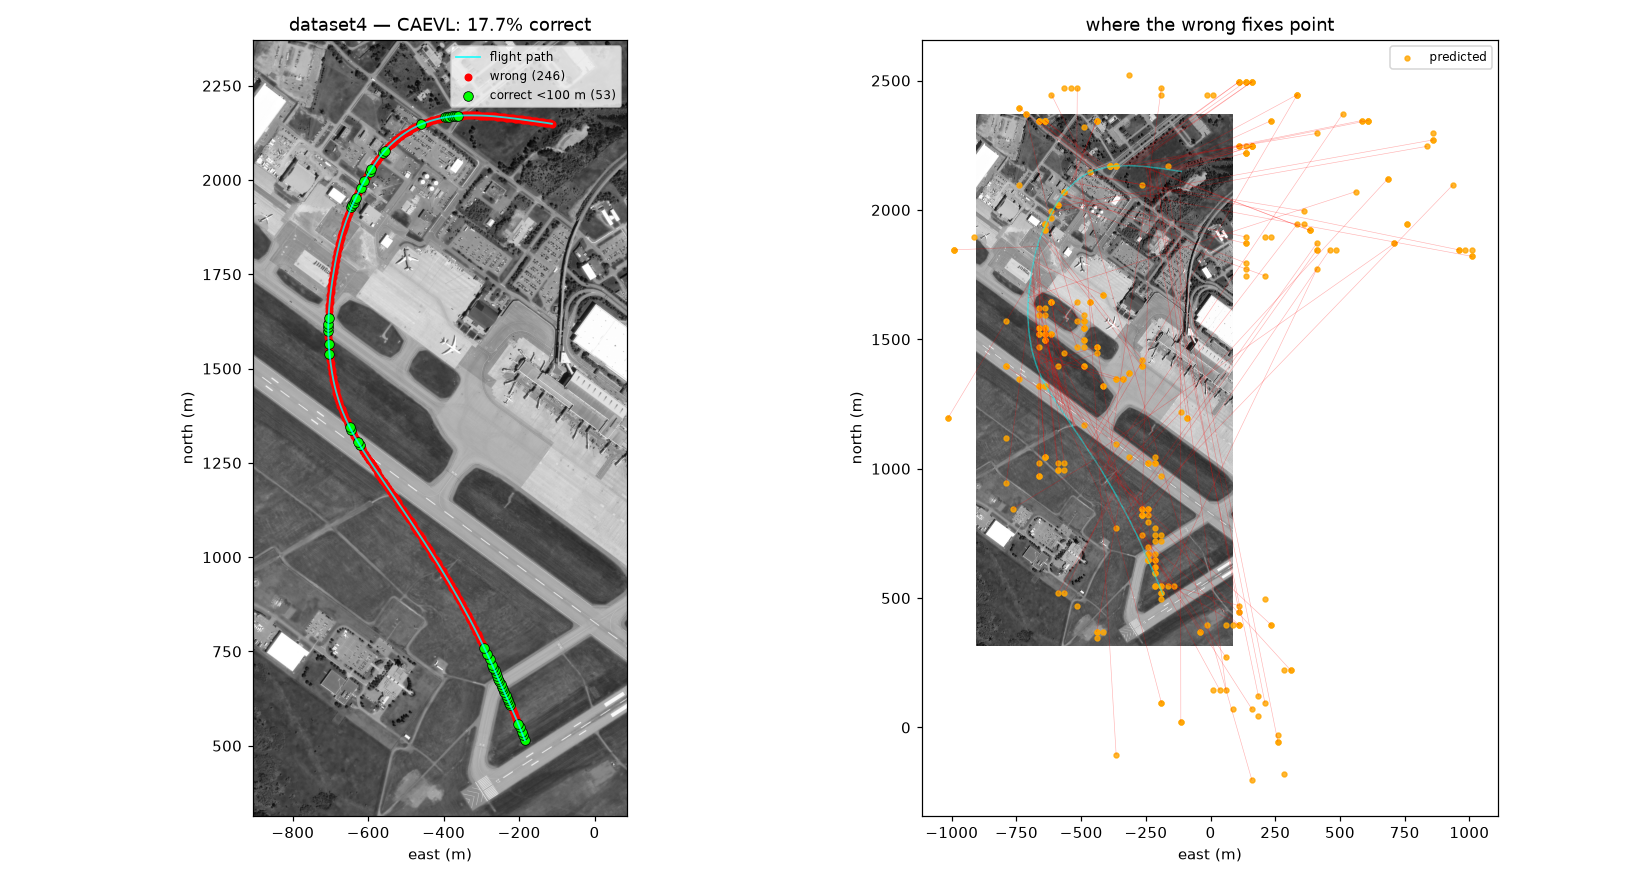
\includegraphics[width=\linewidth]{figures/caevl_dataset4_map.png}

\vspace{0.2em}
{\scriptsize Green = correct. Successes concentrate on runway markings and the
terminal apron; open ground fails.}
\end{column}
\end{columns}
\end{frame}

\begin{frame}{Consensus outlier rejection}
\begin{columns}[T]
\begin{column}{0.44\textwidth}
Wrong predictions scatter roughly uniformly over the map. Two of them agreeing
--- after accounting for the VIO motion between their timestamps --- has
probability
\[
\sim \frac{\pi\tau^2}{A} \approx 0.5\%
\]
Correct ones agree \textbf{by construction}.

\vspace{0.5em}
So: slide a window, RANSAC a similarity transform from two predictions, keep the
largest mutually consistent set.

\vspace{0.5em}
\textbf{Never consults the retrieval score, and never consults the filter's own
belief} --- so it cannot lock itself out.
\end{column}
\begin{column}{0.54\textwidth}
\centering
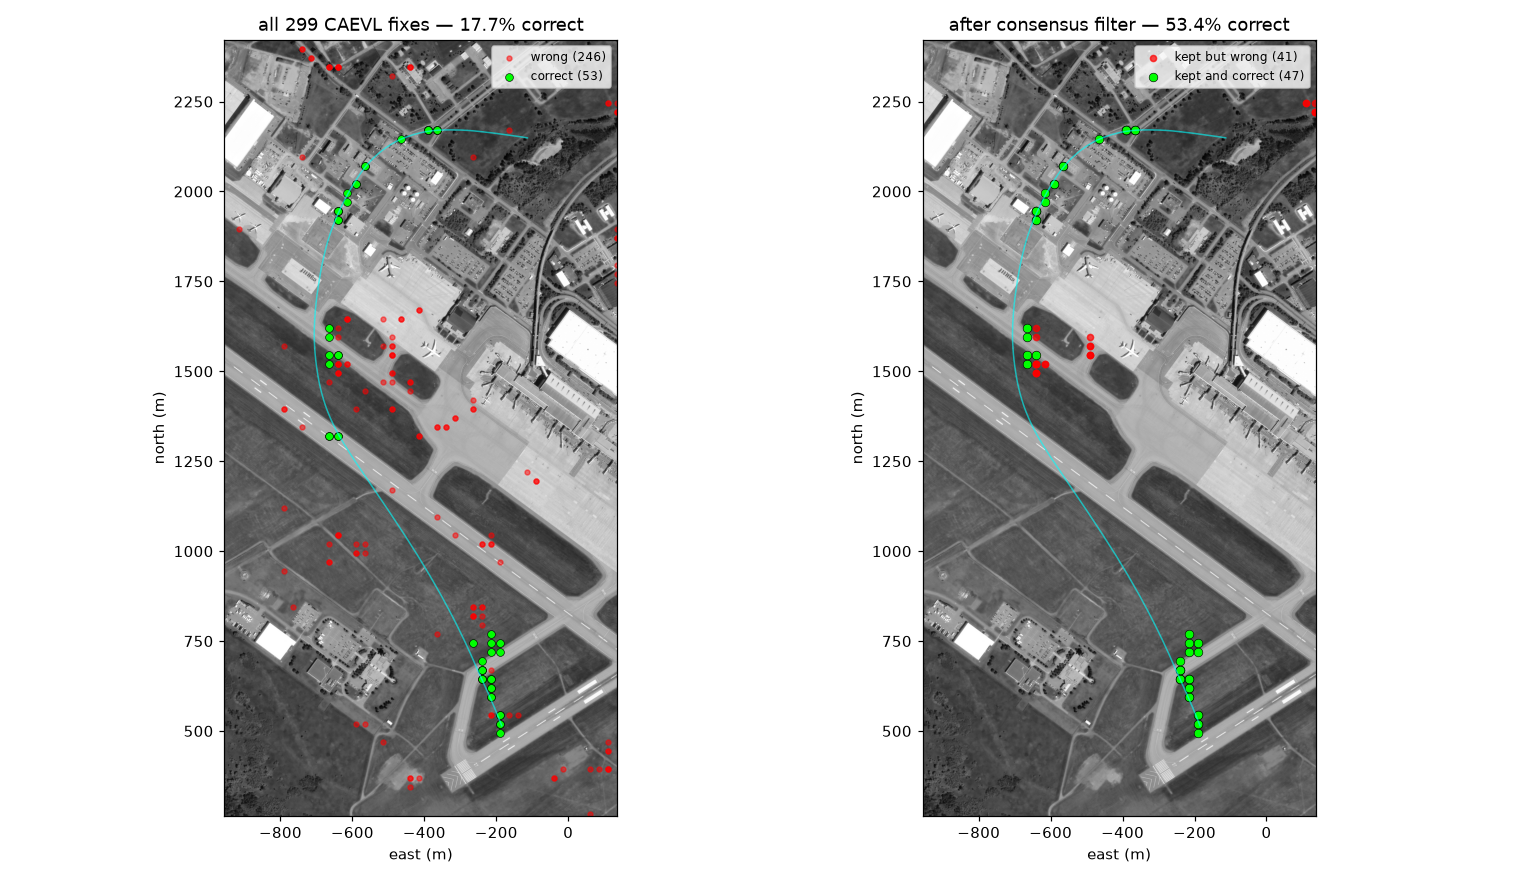
\includegraphics[width=\linewidth]{figures/consensus_filter.png}

\vspace{0.3em}
\begin{tabular}{@{}lcc@{}}
\toprule
 & before & after \\
\midrule
predictions & 299 & 101 \\
precision & 17.7\% & \textbf{99.0\%} \\
correct kept & 107 & 100 (93\%) \\
\bottomrule
\end{tabular}
\end{column}
\end{columns}
\end{frame}

\begin{frame}{Causal fusion}
The VIO trajectory is mapped into the map frame by a similarity transform
estimated \textbf{online, from past predictions only}:
\[
\hat{\bm{p}}_k = s\,\bm{R}(\theta)\,\bm{p}^{\text{vio}}_k + \bm{t}
\]

\vspace{0.3em}
\begin{columns}[T]
\begin{column}{0.5\textwidth}
\textbf{Why estimate $s$ and $\theta$?}
\begin{itemize}
\item OpenVINS initialises with an \textbf{arbitrary heading}
\item Its \textbf{40\% scale deficit} would otherwise reappear between every
      pair of predictions
\end{itemize}

\vspace{0.5em}
\textbf{Before handover:} dead-reckon on the VIO from the known takeoff pose.
A position is output at \textbf{every} instant --- a navigation system cannot
refuse to answer.
\end{column}
\begin{column}{0.5\textwidth}
\textbf{Each step:}
\begin{enumerate}
\item predictions whose timestamp has passed enter a buffer
\item a \emph{trailing} window is screened for consensus
\item survivors accumulate
\item refit $(s,\theta,\bm{t})$ to all accepted history
\end{enumerate}

\vspace{0.4em}
Scale needs a long baseline, so the fit uses the \textbf{full} accepted history
--- still causal, with growing memory.
\end{column}
\end{columns}

\vspace{0.5em}
\footnotesize
\textbf{An EKF over $(x,y,s,\theta)$ with chi-square gating was tried first and
lost}, 422\,m against 347\,m. A scale error makes position error grow
\emph{linearly} while random-walk noise grows as $\sqrt{\cdot}$, so the filter
becomes overconfident and gates out the correct predictions --- most certain
exactly when most wrong. Inflating the covariance reopened the gate and admitted
an outlier that moved the estimate 2.4\,km.
\end{frame}

%---------------------------------------------------------------- 4. results
\begin{frame}{Result --- real-time fusion}
\centering
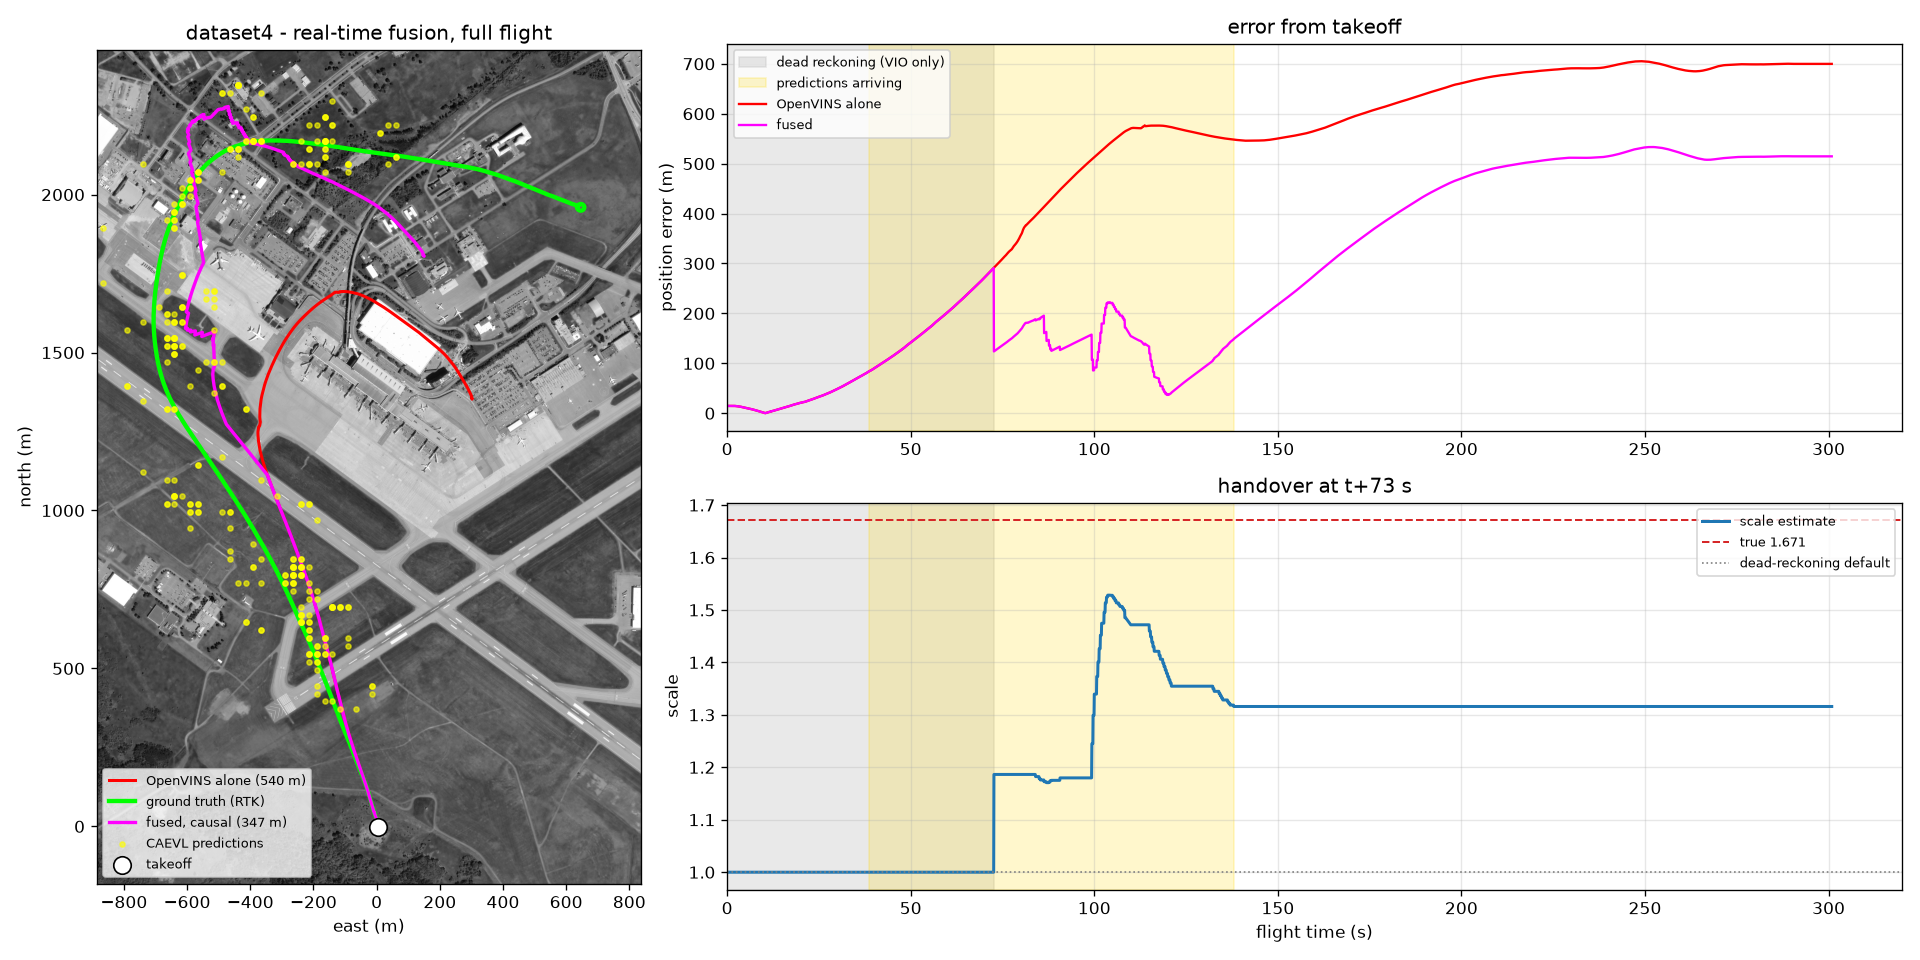
\includegraphics[width=0.93\linewidth]{figures/FINAL_causal_dataset4.png}

\vspace{-0.2em}
{\footnotesize Red: OpenVINS alone. Green: RTK truth. Magenta: fused. Grey:
dead reckoning before handover at $t+73$\,s. \quad
\textbf{540\,m $\rightarrow$ 347\,m}, position output for 100\% of the flight.}
\end{frame}

\begin{frame}{What governs performance}
\begin{columns}[T]
\begin{column}{0.48\textwidth}
\textbf{Scene content, not altitude or database size.}\\
Same aircraft, same airport, same weights:

\vspace{0.3em}
\centering
\begin{tabular}{@{}lc@{}}
\toprule
 & R@100\,m \\
\midrule
dataset3 (forest) & 8.9\% \\
dataset4 (terminal, taxiways) & \textbf{17.7\%} \\
\bottomrule
\end{tabular}

\vspace{0.7em}
\raggedright
\textbf{Search restriction} --- confine the database to the motion prior's
uncertainty region: 5340 $\rightarrow$ 1612 tiles, recall
17.7\% $\rightarrow$ \textbf{35.8\%}.

\vspace{0.4em}
\textbf{Smaller tiles fail.} At 60\,m, 2.21\% of tile pairs exceed 0.99
similarity (vs 0.31\% at 100\,m) --- descriptors collapse.
\end{column}
\begin{column}{0.50\textwidth}
\centering
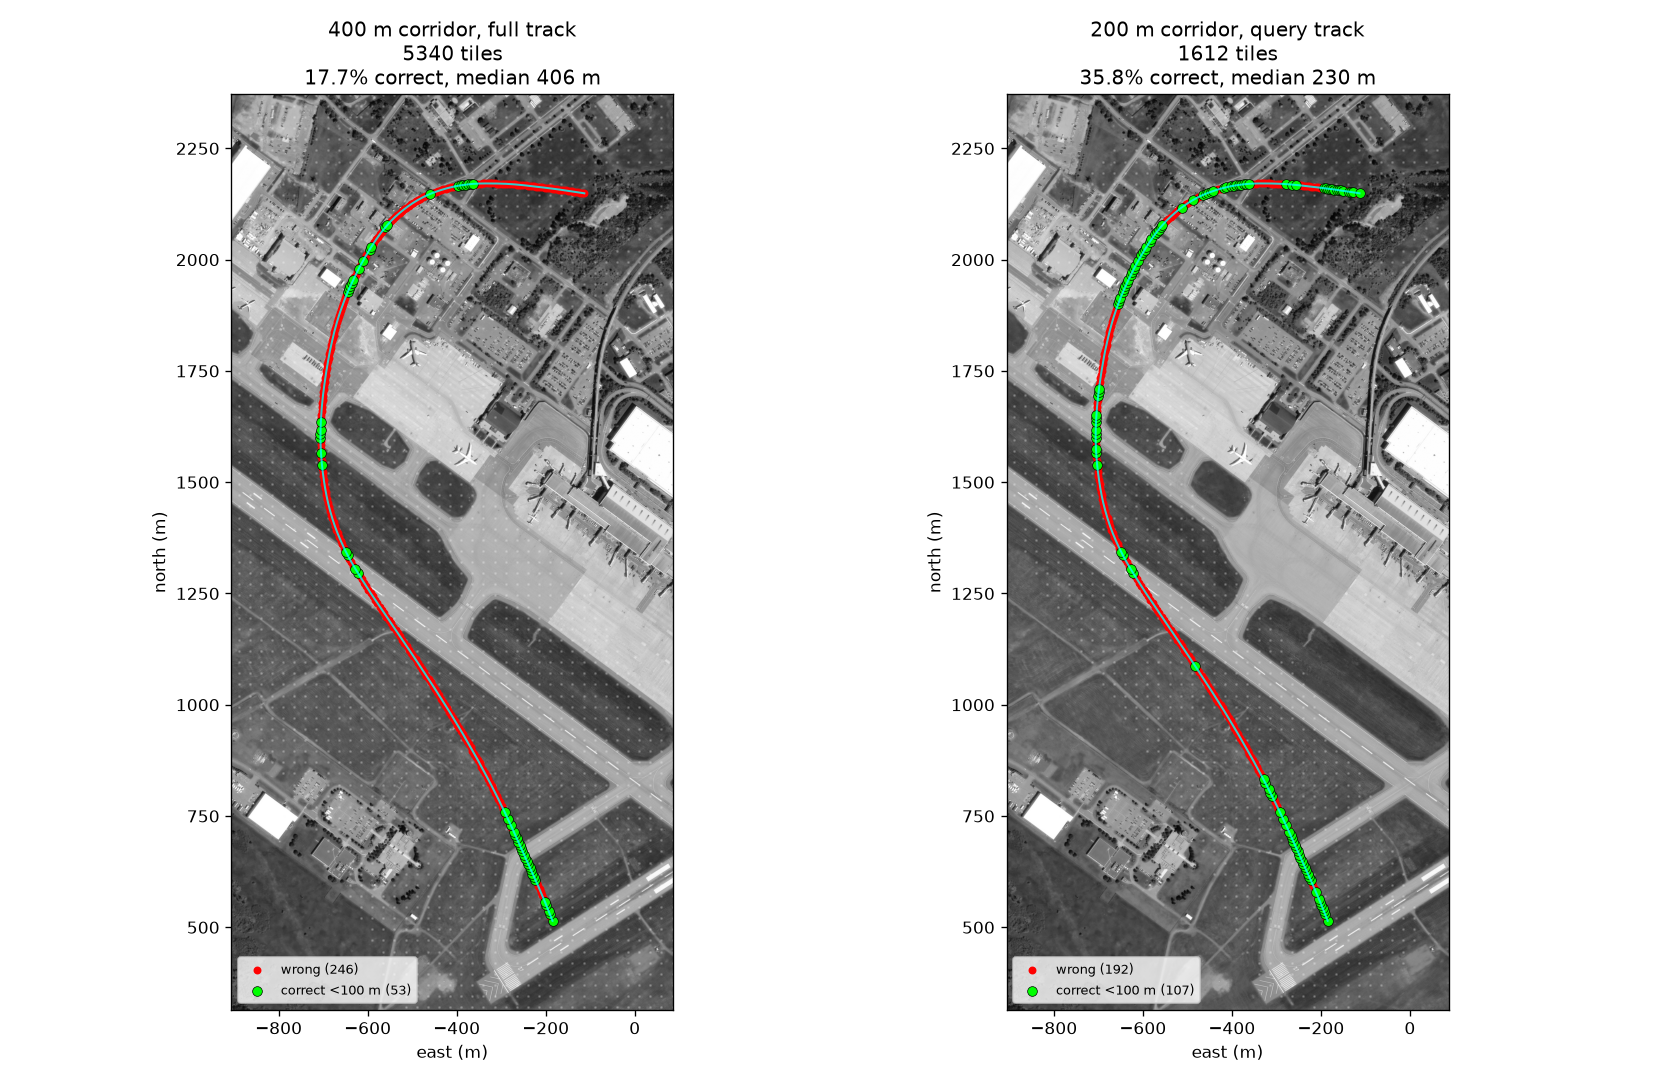
\includegraphics[width=\linewidth]{figures/caevl_q200_compare.png}

\vspace{0.2em}
{\scriptsize Restricting the tile database doubles recall.}
\end{column}
\end{columns}
\end{frame}

\begin{frame}{Limitations and what comes next}
\begin{columns}[T]
\begin{column}{0.52\textwidth}
\textbf{Availability, not accuracy, is the binding constraint.}
\begin{itemize}
\item A 100\,m tile needs $\sim$66\,m of altitude to be imaged. Only \textbf{34\%}
      of this flight is above it.
\item Below that: 1--5\% correct. Tested --- adding those frames made the fusion
      \emph{worse} (347\,m $\rightarrow$ 527\,m).
\item Two quantities still come from ground truth: query \textbf{altitude} and
      initial \textbf{heading}. In deployment: altimeter and magnetometer.
\item Fusion evaluated on one flight; the 40\% VIO scale deficit is unexplained.
\end{itemize}
\end{column}
\begin{column}{0.46\textwidth}
\textbf{Next steps}
\begin{enumerate}
\item \textbf{Query-side scale normalisation} (Shao et al.\ 2026): build one
      database at the lowest operating altitude, rescale queries down to it.
\item \textbf{Retrain CAEVL} at a 100\,m tile footprint instead of ViLD's
      1438\,m --- a $14.4\times$ gap. A training run, not a research problem.
\item Resolve the VIO scale deficit.
\end{enumerate}

\vspace{0.8em}
\centering
\footnotesize
\texttt{github.com/NijatAbbasov06/}\\
\texttt{uav-geolocalization}
\end{column}
\end{columns}
\end{frame}

\end{document}
